\documentclass{article}
\usepackage[utf8]{inputenc}
\usepackage{amsmath}
%\usepackage[norsk]{babel}
\usepackage{amssymb}
\usepackage{tikz}
\usetikzlibrary{decorations.markings}
\usepackage{empheq}
\usepackage{amsthm}
\usepackage{pgfplots}
\usetikzlibrary{decorations.pathreplacing}
\usetikzlibrary{calc}
\usepackage{xcolor}
\usepackage{physics}
\usepackage{fancyhdr}
\pagestyle{fancy}
\usepackage{esdiff}
\usepackage{tikz-feynman}
\usepackage{hyperref}
\usepackage{mathtools}
\usepackage{cleveref}
\usepackage{ulem}
\usepackage{chngcntr}



\title{Lecture notes FY8305}

\date{August, 2019}


\theoremstyle{definition}
\newtheorem{exmp}{Example}[section]

\counterwithin{equation}{section}

\newcommand{\e}{\mathrm{e}}
\newcommand{\dx}{\dd{x}}
\newcommand{\dy}{\dd{y}}
\newcommand{\dxi}{\dd{\xi}}
\newcommand{\dxis}{\dd{\xi^*}}
\newcommand{\Ha}{\mathcal{H}}
\newcommand{\Z}{\mathcal{Z}}

\tikzset{->-/.style={decoration={
  markings,
  mark=at position #1 with {\arrow{>}}},postaction={decorate}}}

\newcommand{\contribs}{%
\begin{center}
\Large 
\textbf{Contributors to the project}
\end{center}


\begin{itemize}
\item Karl Kristian Ladegård Lockert
\item Snorre Bergan
\end{itemize}

%\clearpage
}



\begin{document}

\maketitle
Digitialized from ``FAG 74986 Funksjonal-integral metoder HØST 1996''.
Used as lecture notes for self-study in the course ``FY8305 - Functional Integral Methods in Condensed Matter Physics''. \href{https://www.ntnu.edu/studies/courses/FY8305}{\textbf{Link to course page}}
\contribs
\tableofcontents

\section{Uncertainties/mistakes}

\begin{itemize}
\item Something weird in the derivation of \eqref{unc:statmech}.
\item The indices in equation \eqref{unc:indices} seems off.  
\item In the proof in section \ref{unc:proof} i think there should be a creation operator on one of the last lines in the proof, not annihilation operator as it stands in the notes. $a\e^{\varphi a^\dagger}\ket{0}$ instead of $a\e^{\varphi a}\ket{0}$
\item It is a somewhat unclear purpose of ~\Crefrange{unc:expvalN}{unc:expvalN2}. 
\item The ordering of headlines and equations in section \ref{unc:order_boson} is a bit weird, and some things seem a bit unmotivated. 
\item Double check the labeling on states/ sub indices in \eqref{unc:labeling_on_states} and the previous few eqs. 

\end{itemize}
\section{Short recap of second quantization for fermions and bosons}
Pages 2-10 in lecture notes.

Notation: $ \mu = $ set of quantum numbers that define a one-particle state.


\subsection{Many particle basis}
\newtheorem{theorem}{Ex}
\begin{theorem}


\begin{align*}
\mu &= (\vec{k}, \sigma):\text{Wave number, spin} \\
\mu &= (i, \sigma) : \text{Lattice point, spin} \\
\mu &= (n, i) : \text{Orbital, lattice point} \\
\end{align*}

\end{theorem}

A many-particle basis can be written $\ket{\phi} = \ket{n_{\mu}, n_{\nu}, \dots, n_{\mu_N}}$. Many particle states are built by combining many one-particle states, but where the one-particle states are not necessarily independent. If  \underline{one} of the set of quantum numbers, $\mu_i$, are changed, this \underline{scattering} will generally have consequences for the distribution of quantum numbers for the remaining sets $\{\mu_j\}_{j\ne i}$.
We generally imagine that many-particle states can be built as a linear combination of
$\ket{\phi}$'s;
\begin{equation}
\ket{\Psi} = \sum_{n_{\mu_1},\dots, n_{\mu_N}}\phi_{{\mu_1},\dots, n_{\mu_N}}\ket{{\mu_1},\dots, n_{\mu_N}}.
\end{equation}
A definite one-state vector $\ket{n_{\mu},\dots, n_{\mu_N}}$ can be demanded from a vacuum state (where there is no filled one-particle states) $\ket{0}$ via creation operators.
\begin{align*}
&\textbf{bosons}: &a_\mu^\dagger \\ 
&\textbf{fermions}: &c_\mu^\dagger
\end{align*}


A quanta in a one-particle state can be destroyed by the annihilation operators.

\begin{align*}
&\textbf{bosons}: &a_\mu \\ 
&\textbf{fermions}: &c_\mu
\end{align*}


These operators satisfy some commutation relations:
\begin{align}
&[a_\mu, a_{\nu}] & = [a_\mu^\dagger, a_{\nu}^\dagger] = 0 \\
&[a_\mu, a_{\nu}^\dagger] & = \delta_{\mu\,\nu} \\
&[A,B] &= AB-BA \\
&\{c_\mu^\dagger, c_{\nu}^\dagger\} & = \{c_\mu, c_{\nu}\} = 0 \\
&\{c_\mu, c_{\nu}^\dagger\} & = \delta_{\mu\,\nu} \\
&\{A,B\} &= AB + BA
\end{align}
These will automatically satisfy the Pauli principle as well, which gives \emph{symmetri/ \emph{antisymmetric}} solutions by exchange, dependent if the particles are bosons/fermions. 


\subsection{From classical formulation to second quantization of one-particle operators}

For one-particle operators we usually have a kinetic energy function on a form like
\begin{equation}
T = \sum_i T\left(\vec{r}_i, \vec{p}_i\right) = \sum_i T\left(\vec{r}_i, \diffp{}{r}\right)
\end{equation}
\begin{theorem}
External electrostatic potential:
\begin{equation}
T = \sum_i V_{\text{ext}}\left(\vec{r}_i\right)
\end{equation}
\end{theorem}
\begin{theorem}

Kinetic energy:

\begin{equation}
T = \sum_i \frac{p^2}{2m} = -\sum_i \frac{\hbar^2}{2m}\nabla_i^2
\end{equation}
\end{theorem}

\begin{theorem}
Crystal-potential:
\begin{equation}
T = \sum_i \sum_j v_{\text{cryst}} \left( \vec{r}_i, \vec{R}_j \right)
\end{equation}
\end{theorem}

Second quantization by an operator on this form can be written 
\begin{equation}
T = \sum_{\mu, \nu} T_{\mu\nu}c_\mu^\dagger c_{\nu},
\end{equation}
where
\begin{equation}
T_{\mu\,\nu} = \mel{\mu}{T\left(\vec{r}, \vec{p}\right)}{\nu}.	
\end{equation}

\textbf{Note: The matrix element of one-particle operators are determined by matrix elements in the Hilbert space of one-particle states.}

\subsection{From classical formulation to second quantization of two-particle operators}

Typically, we consider pair-potentials 
\begin{equation}
V = \sum_{i, j} V\left(\vec{r}_i, \vec{r}_j\right).
\end{equation}

\begin{theorem}
Exchange interaction of two charges
\begin{equation}
V = \frac{e^2}{2}\sum_{i\ne j} \frac{1}{|\vec{r}_i - \vec{r}_j|}
\end{equation}
\end{theorem}

The second quantization versions of these are

\begin{equation}
V = \sum_{\mu, \dots, \beta} V_{\mu\nu\alpha\beta}c_{\mu}^\dagger c_{\nu}^\dagger c_{\alpha}c_{\beta},
\end{equation}
where again
\begin{equation}
V_{\mu\nu\alpha\beta} = \mel{\mu\nu}{V\left(\vec{r}_i, \vec{r}_j\right)}{\beta\alpha}
\end{equation}

\textbf{Note: The matrix element of two-particle operators are determined by matrix elements in the Hilbert room of two-particle states.}

The Hamiltonian:
\begin{align}
H &= T + V \label{eq:hamiltonian} \\
T &= -\sum_i \frac{\hbar^2}{2m}\nabla_i^2
\end{align}
So far, we have just presented second quantization for fermion operators, but an equivalent statement will of course hold for the second quantization version of the Hamiltonian for an interacting, material, bosonic system, which has the same identical form as \eqref{eq:hamiltonian}. Notice that each term in $H$ has just as many $c_\mu^\dagger$ as $c_{\nu}$.


\begin{figure}
\centering
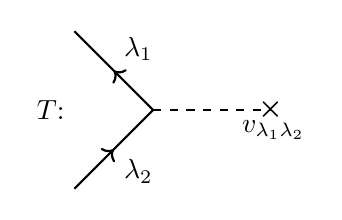
\begin{tikzpicture}

	\draw[thick, ->- = 0.5] (0,0) -- (1,1);
	\draw[thick, ->- = 0.5] (1, 1) -- (0,2);
	\draw[thick, dashed] (1, 1) -- (2.5, 1);
	\node[thick] at (2.5,1){$\cross$};
	\node[anchor = north west, thick] at (0.5, 0.5) {$\lambda_2$};
	\node[anchor = south west, thick] at (0.5, 1.5) {$\lambda_1$};
	\node[anchor = north west, thick] at (2, 1) {$v_{\lambda_1\lambda_2}$};
	\node[anchor = east] at (0, 1) {$T$:};
\end{tikzpicture}
\caption{Scattering from an external potential $v_{\mu\nu}c_{\mu}^\dagger c_{\nu}$}
\end{figure}


\begin{figure}
\centering
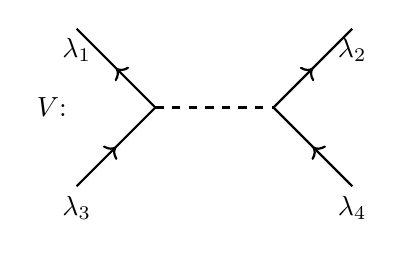
\begin{tikzpicture}

	\draw[thick, ->- = 0.5] (0,0) -- (1,1);
	\draw[thick, ->- = 0.5] (1, 1) -- (0,2);
	\draw[thick, dashed] (1, 1) -- (2.5, 1);
	\draw[thick, ->- = 0.5] (3.5, 0) -- (2.5, 1);
	\draw[thick, ->- = 0.5] (2.5, 1) -- (3.5, 2);
	
	\node[anchor = north] at (0, 0){$\lambda_3$};
	
	\node[anchor = north] at (0, 2){$\lambda_1$};	
	
	\node[anchor = north] at (3.5, 0){$\lambda_4$};

	\node[anchor = north] at (3.5, 2){$\lambda_2$};
	
	\node[anchor = east] at (0, 1) {$V$:};
\end{tikzpicture}
\caption{Exchange interaction between two particles.}
\end{figure}


\subsection{Statistical mechanics}

Assume that we know the spectrum $E_N^n$ for an interacting many-particle system, defined by a state $\ket{\psi_N}_n$, where $N$ is the number of particles in the system and $n$ is an index that indicates what excited state $\ket{\psi_N}_n$ the system is in. 
$\ket{\psi_N}$ is also assumed to be known, such that the matrix product of observables can be calculated: 
\begin{equation}
H\ket{\psi}_n = E_N\ket{\psi}_n.
\end{equation}

To do statistical mechanics, we need to introduce temperature. We do this by using the canonical partition function
\begin{equation}
\label{eq:partition_function}
Z_N = \sum_n\e^{-\beta E_N^n}.
\end{equation}

Note, in \eqref{eq:partition_function} we sum over states, \underline{not} the energy levels $E_N^n$.

\begin{align}
Z &= \sum_n {}_n\mel{\psi_N}{\e^{-\beta H}}{\psi_N}_n \nonumber \\
 &= \Tr\left(\e^{-\beta H}\right) = \Tr\left(S^{-1}S\e^{-\beta H}\right) \nonumber\\
 &= \Tr\left(S\e^{-\beta H}S^{-1}\right) \nonumber \\
 &= \sum_{n'}{}_{n'}\mel{\phi_N}{\e^{-\beta H}}{\phi_N}_{n'}. \label{eq:basis_invariant}
\end{align}

We see in \eqref{eq:basis_invariant} that we can use an \underline{arbitrary} basis to calculate the partition function. The most convenient basis is often a basis where the Hamiltonian is diagonal, but not always.

We write the statistical mean value of an operator as
\begin{align}
\expval{\hat{O}} &\equiv \frac{1}{Z}\Tr\left(\hat{O}\e^{-\beta H}\right) \nonumber\\
&= \frac{1}{Z} \sum_n {}_n\mel{\psi_N}{\hat{O}\e^{-\beta H}}{\psi_N}_n \nonumber \\
&= \frac{1}{Z} \sum_{n, n'} {}_n\expval{\hat{O}}{\psi_N}_{n'}\underbrace{{}_{n'}\expval{\e^{-\beta H}}{\psi_N}_n}_{\delta_{nn'}\e^{-\beta E_{n'}}}.
\end{align}
Thus, we have 
\begin{equation}
\label{eq:expval}
\expval{\hat{O}} = \frac{1}{Z}\sum_n \underbrace{{}_n\expval{\hat{O}}{\psi_N}_n}_{\text{QM matrix element}}\e^{-\beta E_N^n}.
\end{equation}
Notice how the temperature, $T$ only appears in the last factor in \eqref{eq:expval}.
Let us now consider the ground state ($n = 0$) in the low temperature limit with energy $E_0$ corresponding to the state $\ket{\psi_N}_0$.
\begin{align*}
\expval{\hat{O}} &\simeq \frac{1}{Z_{\beta = \infty}}\e^{-\beta E_0} {}_0\expval{\hat{O}}{\psi_N}_0 \\
&= \frac{\e^{-\beta E_0}}{\e^{-\beta E_0}}{}_0\expval{\hat{O}}{\psi_N}_0, 
\end{align*}

such that 
\begin{equation}
\expval{\hat{O}} \stackrel{\beta \rightarrow \infty}{=} {}_0\expval{\hat{O}}{\psi_N}_0.
\end{equation}

We now have a way to calculate the statistical mean value in the ground state at zero temperature. Let us now now assume that the energy spectrum is such that the ground state is separated from excited states by a  \underline{gap} (band insulators, semiconductors, superconductors). This way, we can express the excited state energies as 

\begin{equation}
E_N^1 = E_N^0 + \Delta_N
\end{equation}

such that 
\begin{equation}
E_N^2, E_N^3, \dots \ge E_N^1. 
\end{equation}

This way, we get from \eqref{eq:expval}

\begin{align}
\expval{\hat{O}} &= \frac{1}{Z}\sum_n {}_n\expval{\hat{O}}{\psi_N}_n\e^{-\beta E_N^n} \nonumber\\
&= \frac{\sum_n {}_n\expval{\hat{O}}{\psi_N}_n\e^{-\beta E_N^n}}{\sum_n\e^{-\beta E_N^n}} \nonumber\\
&= \cdots \nonumber\\
% Something fishy right here
&= \frac{{}_0\expval{\hat{O}}{\psi_N}_0\e^{-\beta E_N^0\left(1+\e^{-\beta\Delta}\dots\right)}}{\e^{-\beta E_N^0}\left(1+\e^{-\beta\Delta}\dots\right)} \label{unc:statmech}
\end{align}
and we find that as $\beta\Delta >> 1$, $\hat{O} \simeq {}_0\expval{\hat{O}}{\psi_N}_0$.
In semiconductors we find $\Delta \sim 10\mathrm{mev} \sim 1000\mathrm{K}$.






















\section{Coherent states and Grassman variables}
Pages 10-17 in lecture notes.

\subsection{Coherent states}
A coherent state (both for fermions and bosons) is defined as an eigenstate to an annihilation operator

\begin{align}
	a_\mu \ket{\phi} &= \varphi_\mu \ket{\phi} & \textbf{Bosons}\\
	c_\mu \ket{\psi} &= \xi_\mu\ket{\psi} & \textbf{Fermions}
\end{align}

Both $\ket{\psi}$ and $\ket{\phi}$ must contain a component with the least ($\ge 0$) quantum number (quant), but it is clear that neither $\ket{\psi}$ nor $\ket{\phi}$ can be states with a sharply defined number of particles. They are therefore also ``hard to destroy''. This also explains why we chose to define them as eigenstates of the annihilation operators, not the creation operators. We will get back to the creation of these coherent states. 

We will first look at the bosonic case:
\subsubsection{Bosonic case}

\begin{equation}
a_\mu\ket{\phi} = \varphi_\mu\ket{\phi}
\end{equation}

\begin{align}
[a_\mu, a_{\nu}] = 0& &\nonumber \\
 &\Rightarrow \left(a_\mu a_{\nu} -a_{\nu}a_\mu\right)\ket{\phi} = 0 & \nonumber \\
&= \left(\varphi_\mu\varphi_{\nu} - \varphi_{\nu}\varphi_\mu\right)\ket{\phi} &\nonumber\\
&&\Rightarrow [\varphi_\mu, \varphi_\nu] = 0. \label{eq:coherent_commutator} 
\end{align}

Equation \eqref{eq:coherent_commutator} will always be satisfied if $\varphi_\mu \in \mathbb{C}$. \textbf{The eigenvalues to coherent boson states can be chosen as complex numbers. This is something we can state without knowing anything about how these states are constructed. }

\subsubsection{Fermionic case}
\begin{align}
\{c_\mu, c_\nu\} = 0 && \nonumber \\
&\left(c_\mu c_\nu + c_\nu c_\mu\right)\ket{\psi} = 0 &\nonumber \\
&=\left(\xi_\mu\xi_\nu + \xi_\nu\xi_\mu\right)\ket{\psi} &\nonumber \\
&&\Rightarrow \{\xi_\mu,\xi_\nu\} = 0.\label{eq:coherent_anticommutator}
\end{align}

If $\xi_\mu\in\mathbb{C}$, \eqref{eq:coherent_anticommutator} will only be satisfied if $\{\xi_\mu\} = 0$, trivial eigenvalues. \textbf{The eigenvalues for coherent fermion states must be chosen as anti-commuting numbers, Grassmann-variables.}

\subsection{Grassmann variables}
\subsubsection{Fundamentals}

Equation \eqref{eq:coherent_anticommutator} states the fundamental property of Grassmann variables, and it immediately follows that 
\begin{equation}
\xi_\mu^2 = 0,
\end{equation}
the squares of the Grassmann variables vanish!
Similarly we have that $\xi^n = \xi^2\xi^{n-2} = 0, n \ge 2$.
An arbitrary series expansion in Grassmann variables
\begin{align}
f(\xi) &= \sum_nc_n\xi^n \nonumber \\
&=c_0 + c_1\xi + \dots \nonumber\\
&= x_0 + c_1\xi
\end{align}
is linear.
An arbitrary function of $\xi, \xi^*$ can be written on the forms
\begin{align*}
A\left(\xi, \xi^*\right) &= c_0 + c_1\xi + c_2\xi^*+c_3\xi\xi^* \\
&= c_0 + c_1\xi + c_2\xi^*+d_3\xi^*\xi
\end{align*}

\subsubsection{Grassmann algebra}
We will now look into some of the propreties of functions of Grassmann variable. 

\section{Construction of coherent states for bosons, and its properties}

Pages 18-26 in lecture notes.

\subsection{Construction}
The definition of a coherent boson state $\ket{\phi}$ is stated in \eqref{eq:def_boson_coherent_state}. We make an ansatz -- a qualified guess -- that $\ket{\phi}$ can be created as
\begin{equation}
\label{eq:construction_coherent_boson}
\ket{\phi} = \e^{\sum_\mu\varphi_\mu a_\mu^\dagger}\ket{0}.
\end{equation}

We claim that 
\begin{equation}
\label{unc:indices}
a_\mu\e^{\sum_\nu\varphi_\nu a_\nu^\dagger}\ket{0} = \varphi_\mu\e^{\sum_\nu\varphi_\nu a_\nu^\dagger}\ket{0}
\end{equation} % TODO: CHECK THIS

\begin{proof}
\label{unc:proof}
\begin{equation*}
a\sum_{n=0}\frac{\left(\varphi a^\dagger\right)^n}{n!}\ket{0} = a\sum_{n=1} \frac{\varphi^n}{n!}\left(a^\dagger\right)^n\ket{0}.
\end{equation*}
Note that $\left(a^\dagger\right)^na\ket{0} = 0$, and so we wish to ``commute $a$ through''.

\begin{align*}
\comm{a}{f\left(a^\dagger\right)} &= \sum_{n=1}c_n\comm{a}{\left(a^\dagger\right)^n} \\
&= \sum_{n=1}nc_n\left(a^\dagger\right)^{n-1}\\
f\left(a^\dagger\right) &= \sum_{n=0}^\infty c_n\left(a^\dagger\right)^n \\
&\implies \comm{a}{f\left(a^\dagger\right)} = \pdv{a^\dagger}f\left(a^\dagger\right).
\end{align*}

More generally:

\begin{align*}
\comm{g(a)}{f(a^\dagger)} &= g\left(\pdv{a^\dagger}\right)f\left(a^\dagger\right)\\
\comm{a}{\left(a^\dagger\right)^n} &= n\left(a^\dagger\right)^{n-1} \\
\comm{\left(a\right)^m}{\left(a^\dagger\right)^n} &= \frac{n!}{(n-m)!}\left(a^\dagger\right)^{n-m} \\
\acomm{c}{f\left(c^\dagger\right)} &= \pdv{c^\dagger}f\left(c^\dagger\right) \\
\acomm{g(c)}{g(c^\dagger)} &= g\left(\pdv{c^\dagger}\right)f\left(c^\dagger\right)
\end{align*}

To find out what the commutator $\comm{a}{\left(a^\dagger\right)^n}$ is, we use that 
\begin{equation}
\comm{A}{BC} = \comm{A}{B}C + B\comm{A}{C}, 
\end{equation}
with $A =a, B = a^\dagger, C = \left(a^\dagger\right)^{n-1}$ to get

\begin{align*}
\comm{a}{\left(a^\dagger\right)^n} &= \left(a^\dagger\right)^{n-1} + a^\dagger\comm{a}{\left(a^\dagger\right)^{n-1}} \\
&= a\left(a^\dagger\right)^{n-1} \\
\implies a\left(a^\dagger\right)^{n}\ket{0} &= n\left(a^\dagger\right)^{n-1}\ket{0}\\
\implies a\e^{\varphi a^\dagger}\ket{0} &= \sum_{n=1}^\infty\frac{\varphi^nn\left(a^\dagger\right)^{n-1}}{n!}\ket{0} \\
&= \varphi\sum_{n=1}^\infty\frac{\left(\varphi a^\dagger\right)^{n-1}}{(n-1)!}\ket{0}\\ &= \varphi\e^{\varphi a^\dagger}\ket{0}.
\end{align*}
\end{proof}

Then, for more modes (quantum numbers), we get
\begin{equation}
\ket{\phi} = \e^{\sum_\mu\varphi_\mu a_\mu^\dagger}\ket{0}
\end{equation}
with the $\varphi_\mu$'s satisfying
\begin{equation}
a_\mu\ket{\phi} = \varphi_\mu\ket{\phi}.
\end{equation}
Coherent states: ``difficult to destroy''.

We also could have done this in a more direct way:
Assume
\begin{equation}
\ket{\phi} = \prod_\mu f_\mu\left(\varphi, a_\mu^\dagger\right)\ket{0}
\end{equation}
with 
\begin{equation}
a_\mu =\varphi_\mu\ket{\phi}.
\end{equation}

Then, we need that 
\begin{equation}
a_\mu f_\mu\left(\varphi, a_\mu^\dagger\right)\ket{0} = \varphi_\mu f_\mu\left(\varphi, a_\mu^\dagger\right)\ket{0},
\end{equation}

but

\begin{align}
a_\mu f_\mu \ket{0} &= \comm{a_\mu}{f_\mu}\ket{0}\\
&\implies \pdv{a_\mu^\dagger} f_\mu = \varphi_\mu f_\mu \\
\implies \frac{\dd{f_\mu}}{{f_\mu}} &= \varphi_\mu \dd{a_\mu^\dagger} \\
\ln f_\mu &= \varphi_\mu a_\mu^\dagger \\
f_\mu &= \e^{\varphi_\mu a_\mu^\dagger}.
\end{align}

\subsection{Properties}
We will now look at some of the properties of coherent bosonic states. 
\begin{align}
a_\mu^\dagger\ket{\phi} &= a_\mu^\dagger\e^{\sum_\mu\varphi_\nu a_\nu^\dagger}\ket{0}\\
&= \pdv{\varphi_\mu}\ket{\phi}
\end{align}

\begin{align}
\bra{\phi} &= \bra{0}\e^{\sum_\mu \varphi_\mu^*a_\mu} \implies\\
\bra{\phi}a_\mu &= \pdv{\varphi_\mu^*}\bra{\phi}
\end{align}

The overlap of two coherent bosonic states are
\begin{equation}
\braket{\phi}{\sigma} = \mel{0}{\e^{\sum_\mu\varphi_\mu^*a_\mu}\e^{\sum_\nu\sigma_\nu a_\nu^\dagger}}{0}.
\end{equation}

Now define 
\begin{align*}
A &= \sum_\mu\varphi_\mu^*a_\mu \\
B &= \sum_\nu\sigma_\nu a_\nu
\end{align*}

such that 
\begin{equation}
\braket{\phi}{\sigma} = \mel{0}{\e^{A}\e^{B}}{0}.
\end{equation}

We see that 
\begin{equation}
\mel{0}{\e^{B}\e^{A}}{0} = 1.
\end{equation}

Baker-Hausdorff:
\begin{align}
e^{A+B} &=\e^{A}\e^{B}\e^{-\frac{1}{2}\comm{A}{B}} \\
		&= \e^{B}\e^{A}\e^{-\frac{1}{2}\comm{B}{A}},
\end{align}

where $\comm{A}{B}$ commutes with $A, B$.
\begin{align}
\implies \e^A\e^B &= \e^B\e^A\e^{\comm{A}{B}} \\
\comm{A}{B} &= \sum_{\mu,\nu}\varphi_\mu^*\sigma_\nu\underbrace{\comm{a_\mu}{a_\nu^\dagger}}_{\delta_{\mu\nu}} \\
	&= \sum_\mu\varphi_\mu^*\sigma_\mu \\
	\implies& \\
	 \braket{\phi}{\sigma} &= \e^{\sum_\mu\varphi_\mu^*\sigma_\mu}\underbrace{\mel{0}{\e^B\e^A}{0}}_{=1}\\
	 &= \e^{\sum_\mu\varphi_\mu^*\sigma_\mu},
\end{align}
the states are not orthogonal!

For the normalization of \(\ket{\phi}\) we have
\begin{align}
\braket{\phi} &= \e^{\sum_\mu\varphi_\mu^*\varphi_\mu} \\
	&= \e^{\ev{N}}.
\end{align}
\(\ev{N}\) is the average number of particles in the state \(\ket{\phi}\)

\begin{align}\label{unc:expvalN}
\frac{\ev{\sum_\mu a_\mu^\dagger a_\mu}{\phi}}{\braket{\phi}} &= \ev{N} \\
&= \sum_\mu \varphi_\mu^*\varphi_\mu
\end{align}

\begin{align}
\ev{\left(\Delta N \right)^2} &= \frac{1}{\braket{\phi}}\left[ \ev{\hat{N}^2}{\phi} - \left( \ev{\hat{N}}{\phi}\right)^2\right] \\
&= \frac{1}{\braket{\phi}}\left[\ev{\sum_{\mu, \nu}a_\mu^\dagger a_\mu a_\nu^\dagger a_\nu}{\phi} - \left(\sum_\mu\varphi_\mu^*\varphi_\mu\right)^2\right]\\
\label{unc:expvalN2}
&= \sum_\mu\varphi_\mu^*\varphi_\mu = N.
\end{align}

\subsection{Coherent states for a one-bosonic oscillator}

Following the construction from \eqref{eq:construction_coherent_boson}, we have
\begin{align}
\ket{z} &= \e^{za^\dagger}\ket 0 \\
&= \sum_{n=0}^\infty \frac{z^n\left(a^\dagger\right)^n}{n!}\ket{0} = \sum_n \frac{z^n}{\sqrt{n!}}\frac{\left(a^\dagger\right)}{\sqrt{n!}}\ket 0 \\
&= \sum_n\frac{z^n}{\sqrt{n!}}\ket n
\end{align}

\begin{align}
\label{eq:completeness_coherent_boson}
&\frac{1}{2\pi i}\int\dd z \dd{z^*}\e^{-z^*z}\dyad z \\
&= \frac{1}{2\pi i}\int \dd z \dd{z^*}\e^{-zz^*}\sum_{n,m}\frac{z^n}{\sqrt{n!}}\frac{\left(z^*\right)^m}{\sqrt{m!}}\dyad m \\
&= \frac{1}{2\pi i}\sum_{n, m}\frac{1}{\sqrt{n!m!}}\dyad{n}{m}\int\dd z \dd{z^*}\e^{-zz^*}z^n\left(z^*\right)^m \\
&= \frac{1}{\pi}\sum_{n, m}\frac{1}{\sqrt{n!m!}}\dyad{n}{m}\int \dd{x}\dd{y} \e^{-\left(x^2 + y^2\right)}\left(x+iy\right)^n)\left(x-iy\right)^m. \label{eq:coherent_state_integral}
\end{align}
Now, the integral in \eqref{eq:coherent_state_integral} is
\begin{align}
&\frac{1}{\pi}\int\dx\dy\e^{-\left(x^2 + y^2\right)}\left(x+iy\right)^n)\left(x-iy\right)^m \nonumber \\
&= \frac{1}{\pi} \int \dd{\rho}\rho\dd{\theta}\e^{-\rho^2}\left(\rho\e^{i\theta}\right)^n\left(\rho\e^{-i\theta}\right)^m\nonumber \\
&= \frac{1}{\pi}\underbrace{\int\dd{\theta}\e^{i\theta(n-m)}}_{2\pi\delta_{nm}}\int\dd{\rho}\rho^{n+m+1}\e^{-\rho^2}\nonumber \\
&= 2\delta_{nm}\int\dd{\rho}\rho^{2n+1}\e^{-\rho^2}\nonumber\\ 
&= \delta_{nm}\int_0^\infty\dd{r}r^{-\frac{1}{2}}r^{\frac{2n+1}{2}}e^{-r} = \int_0^\infty\dd{r}r^n\e^{-r} \nonumber\\
&= \delta_{nm}n!,
\end{align}
such that \eqref{eq:completeness_coherent_boson} becomes

\begin{align*}
\frac{1}{2\pi i}\int\dd z \dd{z^*}\e^{-z^*z}\dyad z &= \sum_{n, m}\frac{1}{\sqrt{n!m!}}\dyad{n}{m}\cdot \delta_{nm}n! \\
&= \sum_{n}\dyad{n} = 1.
\end{align*}
\section{Coherent states for fermions}

\subsection{Construction}

We will also in the fermionic case make an ansatz on the construction of coherent fermionic states, somewhat similar to \eqref{eq:construction_coherent_boson}:
\begin{align}
\ket \psi &= \e^{-\sum_\mu\xi_\mu c_\mu^\dagger}\ket 0 \\
&= \prod_\mu \left(1-\xi_\mu c_\mu^\dagger\right)\ket 0
\end{align}

It is simpler to show that the ansatz satisfies the definition \eqref{eq:def_fermion_coherent_state} ( \( c_\mu \ket{\psi} = \xi_\mu\ket{\psi}\) ) for fermions than it was for bosons. Use the fact that \(\xi_\mu^2 = 0\) to express the expansion of the exponential function. 
\begin{equation}
c_\mu\prod_\nu\left(1-\xi_\nu c_\nu^\dagger\right)\ket 0 = c_\mu \ket \psi
\end{equation}
affects one of the products:
\begin{align}
c_\mu\left(1-\xi_\mu c_\mu^\dagger\right)\ket 0 &= +\xi_\mu \underbrace{c_\mu c_\mu^\dagger}_{1-c_\mu\dagger c_\mu}\ket 0 \\
&= +\xi_\mu \ket 0  \\
&= \xi_\mu\left(1-\xi_\mu c_\mu^\dagger\right)\ket 0 \\
&\implies \nonumber\\
 &c_\mu\ket \psi = \xi_\mu\ket\psi,
\end{align} 

where we used the anticommutation relations \(\acomm{\xi_\mu}{c_\mu} = \acomm{\xi_\mu}{c_\mu^\dagger} =0\).

\subsection{Properties}
\subsubsection*{Creation operator}
Acting with the creation operator on a coherent fermion state:
\begin{align*}
c_\mu^\dagger\ket\psi &= c_\mu^\dagger\left(1-\xi_\mu c_\mu^\dagger\right)\prod_{\nu \ne \mu}\left(1-\xi_\nu c_\nu^\dagger\right)\ket 0\\
&= -\pdv{\xi_\mu}\left(1-\xi_\mu c_\mu^\dagger\right)\prod_{\nu \ne \mu}\left(1-\xi_\nu c_\nu^\dagger\right)\ket 0 \\
&= -\pdv{\xi_\mu}\ket \psi.
\end{align*}

Similarly, on the ``bra'' vectors:
\begin{align*}
\bra\psi c_\mu &= \prod_{\mu}\bra 0 \left(1+\xi_\mu^*c_\mu\right)c_\mu \\
&=\pdv{\xi_\mu^*}\prod_{\mu}\bra 0 \left(1+\xi_\mu^*c_\mu\right)\\
&= \pdv{\xi_\mu^*}\bra\psi
\end{align*}
NB: Note the plus sign in the product.

\subsubsection*{Overlap}
The overlap between two coherent fermion states:

\begin{align*}
\braket{\psi}{\psi'} &= \mel{0}{\prod_{\mu, \nu}\left(1+\xi_{\nu}^*c_{\nu}\right)\left(1-\xi_\mu c_\mu^\dagger\right)}{0} \\
&= \prod_{\mu, \nu}\mel{0}{\left(1+\xi_{\nu}^*c_{\nu}\xi_\mu c_\mu^\dagger\right)}{0}\\
&=\prod_{\nu \ne \mu}\cdot 1 \prod_{\mu}\left(1+\xi_\mu^*\xi_\mu\right) \\
&= \prod_{\mu}\left(1+\xi_\mu^*\xi_\mu\right) \\
\text{Re-exponentiation} \implies \braket{\psi}{\psi'} &= \e^{\sum_\mu\xi_\mu^*\xi_\mu}.
\end{align*}
We have used \(\acomm{c_\mu}{\xi_\mu}=0\).

\subsubsection*{Completeness relation}

The completeness relation for fermion coherent states is
\begin{equation}
\int \prod_{\mu}\dd{\xi_\mu^*}\dd{\xi_\mu \e^{-\sum_\mu\xi_\mu^*\xi_\mu}}\dyad{\xi} = 1.
\end{equation}

\begin{proof}
\underline{\textbf{For one mode:}}
\begin{align*}
&\int \dxi\dxis\e^{-\xi^*\xi}\e^{-\xi c^\dagger}\dyad 0\e^{-c\xi^*}& \\
&=\int \dxi\dxis \left(1-\xi^*\xi\right)\left(1-\xi c^\dagger\right)\dyad 0 \left(1-c\xi^*\right)\\
&=\int \dxi\dxis \left[1-\xi^*\xi -\xi ^\dagger\right]\dyad 0 \left(1+\xi^* c\right)\\
&=\int \dxi\dxis\left[\left(1-\xi^*\xi\right)\ket 0 - \xi c^\dagger \ket 0\right]\left[\bra 0 + \xi^*\bra 0 c\right] \\
&= \int \dxi\dxis \left[\left( 1-\xi^*\xi\right)\dyad 0 -\xi c^\dagger \dyad 0 \right. \\
&\qquad\qquad\quad +\left.\left(1-\xi^*\xi\right)\ket 0\xi^*\bra 0 c - \xi c^\dagger\ket 0\xi^*\bra 0 c\right] \\
&=\int \dxi\dxis \left[\left(1-\xi^*\xi\right)\dyad 0 -\xi \dyad{1}{0} \right.\\
&\qquad\qquad\quad +\left.\left(1-\xi^*\xi\right)\xi^*\dyad{0}{1} + \xi\xi^* \dyad 1\right]\\
&= \dyad 0 + \dyad 1 = 1
\end{align*}

\underline{\textbf{For multiple modes:}}

\begin{align*}
&\int \prod_\mu \dxi_\mu \dxis_\mu \e^{-\sum_\mu \xi_\mu^* \xi_\mu}\dyad \xi \\
&=\int \prod_\mu\dxi_\mu\dxis\mu\e^{-\sum_\mu\xi_\mu^*\xi_\mu}\e^{-\sum_\mu\xi_\mu c_\mu^\dagger}\dyad 0\e^{-\sum_\mu c_\mu\xi_\mu^*}\\
&= \int \left(\prod_{\mu}\dd{\xi_\mu^*}\dd{\xi_\mu}\right)\left(\prod_\mu\left(1-\xi_\mu^*\xi_\mu\right)\right)\left(\prod_\mu\left(1-\xi_\mu c_\mu^\dagger\right)\right) \\
&\qquad\qquad\quad \times \dyad 0 \left(\prod_\mu\left(1+\xi_\mu^* c_\mu\right)\right)
\end{align*}
We can treat \(\xi_\mu^*\xi_\mu, \xi_\mu c_\mu^\dagger\) etc. as ordinary numbers when we change places, since they commute.

\end{proof}

The trace of an operator:
\begin{align}
\label{eq:Trace_fermion_coherent}
\Tr A =&\sum_n\ev{A}{n} \nonumber \\
&= \int \prod_{\mu}\dd{\xi_\mu^*}\dd{\xi_\mu \e^{-\sum_\mu\xi_\mu^*\xi_\mu}}\sum_n\braket{n}{\xi}\mel{\xi}{A}{n}\nonumber \\
&=\int \prod_{\mu}\dd{\xi_\mu^*}\dd{\xi_\mu \e^{-\sum_\mu\xi_\mu^*\xi_\mu}}\underbrace{\sum_n \mel{-\xi}{A}{n}\braket{n}{\xi}}_{\mel{-\xi}{A}{\xi}} \nonumber\\
&=\int \prod_{\mu}\dd{\xi_\mu^*}\dd{\xi_\mu \e^{-\sum_\mu\xi_\mu^*\xi_\mu}}\mel{-\xi}{A}{\xi} 
\end{align}

\(\hat{N} = \sum_\mu c_\mu^\dagger c_\mu\)is the number operator, as usual. What is the mean value of this operator in a fermion coherent state?

\begin{align}
\frac{\ev{\hat{N}}{\xi}}{\braket{\xi}} &= \sum_\mu \frac{\ev{c_\mu^\dagger c_\mu }{\xi}}{\braket \xi} \\
&= \sum_\mu \xi_\mu^* \xi_\mu 
\end{align}
This is neither a real nor complex number! It is therefore meaningless to talk about the mean value of number of fermions in a coherent state. 

In \eqref{eq:Trace_fermion_coherent} we used a property that is not true in general, but is under the integral.
\begin{align*}
\braket{\psi}{\xi} &= c_0 + c_1\xi \\
\braket{\xi}{\psi} &= d_0 + d_1\xi^*
\end{align*}
Terms linear in \(\xi, \xi^*\) is zero under Grassmann integration
\begin{align*}
\ket \xi &\equiv \e^{\xi c^\dagger}\ket 0\\
\ket{-\xi} &= \e^{-\xi c^\dagger}\ket 0 \\
&\ne -\ket \xi
\end{align*}
Such that 
\begin{equation}
\braket{\psi}{\xi}\braket{\xi}{\psi} \ne \braket{-\xi}{\psi}\braket{\psi}{\xi},
\end{equation}

but it comes out correct in the integral. We used this as

\begin{equation}
\int\dd{\xi}\dd{\xi^*}\braket{\psi}{\xi}\braket{\xi}{\psi} = \int\dd{\xi}\dd{\xi^*}\braket{-\xi}{\psi}\braket{\psi}{\xi}
\end{equation}

The reason for this fundamental difference between Bosonic and fermionic coherent states lies in the Pauli exclusion principle and the definition of coherent states.

With a \underline{given set} of one-particle states, together with the Pauli princliple, a physical state must have a fixed, determinable number of particles, and cannot be an eigenstate of a annihilation operator. The fermionic coherent states therefore lay outside the Hilbert space of physical states, and need not represent observable states. For bosons, the symmetric property means that even with a \underline{given set} of quantum numbers, physical states can be an eigenstate of the annihilation operator. This is because each one particle state can assume an arbitrary number of quants. Boson coherent states are thus \underline{physical}. They are in fact physical states naturally occurring when taking the classical limit of a quantum field theory. Also in lasers. 

When we considered the trace (eq \eqref{eq:Trace_fermion_coherent} ) of an operator \(A\) for both for both fermionic and bosonic coherent states, we had to consider the matrix elements

\begin{align*}
	\mel{\phi}{A}{\phi} && \textbf{(Bosons)}\\
	\mel{-\psi}{A}{\psi} && \textbf{(Fermions)} 
\end{align*}

For bosons: Assume that \(A(a_\mu^\dagger, a_\mu)\) are normal ordinals \label{unc:ordinals}; all \(a_\mu\) are placed to the right of \(a_\mu^\dagger\)-

\begin{align}
a_\mu\ket\phi &= \varphi_\mu\ket\phi \\
\left(a_\mu\right)^n\ket\phi &= \left(\varphi_\mu\right)^n\ket\phi \\
A\left(a_\mu\right)\ket\phi &= A\left(\varphi_\mu\right)\ket\phi,
\end{align}
thus

\begin{align}
\mel{\phi}{A\left( a_\mu^\dagger, a_\mu\right)}{\phi'}
&= A\left(\varphi_\mu^*, \varphi_{\mu'}\right)\braket{\phi}{\phi'} \\
&= A\left(\varphi_\mu^*, \varphi_{\mu'}\right)\e^{\sum_\mu\varphi_\mu^*\varphi_{\mu'}}. 
\end{align}
Similarly, 

\begin{equation}
\label{unc:labeling_on_states}
\mel{\psi}{A\left( c_\mu^\dagger,c_\mu\right)}{\psi'} = A\left(\xi_\mu^*,\xi_\mu'\right)\e^{\sum_\mu\xi_\mu^*\xi_\mu'}
\end{equation}

Thus, the calculation of expectation values reduces to quadratures; multiple integrals over \((\varphi_\mu^*, \varphi_\mu)\) or \((\xi_\mu^*, \xi_\mu)\).
\section{Free electron gas}
\label{sec:free_electron}

We start with the Hamiltonian
\begin{align}
\Ha &= \sum_{k,\sigma}\varepsilon_kc_{k\sigma}^\dagger c_{k\sigma}\nonumber \\
& = \sum_\sigma \int \dx \psi_\sigma^\dagger(x)\varepsilon(\nabla)\psi_\sigma(x).
\end{align}
The partition function is 

\begin{equation}
\label{eq:partition_integral}
\Z = \int \mathcal{D}\left[\varphi^*(\tau)\right]\mathcal{D}\left[\varphi(\tau)\right]\e^{\mathcal{S}}
\end{equation}
where \( \varphi_\lambda(0) = -\varphi_\lambda(\beta)\) (antiperiodic for fermions) and
\begin{equation}
\mathcal{S} = -\sum_\lambda\int_0^\beta\dd{\tau}\left[\varphi_\lambda^*\pdv{\varphi_\lambda}{\tau} + \Ha \left(\{\varphi_\lambda^*, \varphi_\lambda\}\right)\right]
\end{equation}
Now choose quantum numbers \(\lambda = \left(k,\sigma\right)\) because $\Ha$ is diagonal in the plane wave basis. Then,  
\begin{equation}
\mathcal{S} = -\sum_{k,\sigma}\int_0^\beta\dd{\tau}\varphi_{k\sigma}^*(\tau)\left(\pdv{\tau} + \varepsilon_k\right)\varphi_{k\sigma}(\tau)
\end{equation}
where $\{\varphi_{k\sigma}(\tau)\}$ are Grassman variables. $\Z$ now becomes a Gaussian integral over Grassmann variables, which we have seen earlier. By direct insertion of this result, we find 

\begin{align}
\Z &= \e^{\Tr \ln\left(\partial_\tau + \varepsilon_k\right)} \label{eq:partition_free_electron}\\
&\stackrel{?}{=} \prod_{k,\sigma}\left(1+\e^{-\beta\varepsilon_k}\right)\nonumber
\end{align} 
with 
\begin{equation}
\label{eq:trace_}
\Tr = \sum_{k,\sigma}\int_0^\beta\dd{\tau}\cdot \tr
\end{equation}
where ``tr'' here is the trace of the operator $\ln\left(\partial_\tau + \varepsilon_k\right)$
\begin{equation}
\tr\ln\left(\partial_\tau + \varepsilon_k\right) = \sum_n\ev{\ln\left(\partial_\tau + \varepsilon_k\right)}{n}.
\end{equation}
To be able to get a \underline{local} expression for $\ln\left(\partial_\tau + \varepsilon_k\right)$, the choice of a plane wave basis for $\ket n$ is convenient.

\begin{equation}
\ket n = u_{nk} = \frac{1}{\sqrt{\beta}}\e^{i\left(\textbf{k}\cdot\textbf{r} - \omega_n\tau \right)}
\end{equation}
where
\begin{equation}
\omega_n = \frac{\left(2n+1\right)\pi}{\beta}.
\end{equation}
The reason for this choice of $\omega_n$ is that we see that this ensures $u_{nk}(\tau)$ to have the same \underline{antiperiodic} properties as $\varphi_\lambda(\beta)$
When we take the trace only over such states, the requirement \( \varphi_\lambda(0) = -\varphi_\lambda(\beta)\) is automatically satisfied.

\begin{align}
&\sum_n \ev{\ln\left(\partial_\tau + \varepsilon_k\right)}{n} & \nonumber \\
& = \frac{1}{\beta}\sum_{\omega_n}\e^{-i\left(\textbf{k}\cdot \textbf{r} - \omega_n\tau\right)}\ln\left(\partial_\tau + \varepsilon_k\right)\e^{i\left(\textbf{k}\cdot \textbf{r} - \omega_n\tau\right)}. \label{eq:trace_free_electron}&
\end{align}

Before we continue, we investigate the trace of an arbitrary operator
\begin{equation}
\tr\ln A = \sum_n\ev{A}{n}.
\end{equation}

$\ln A$ is defined by its series expansion

\begin{align}
\ln A &= \ln (1+A-1) \nonumber \\
&= \sum_{k=1}^\infty\frac{(-1)^{k+1}}{k}\left(A-1\right)^k,
\end{align}
such that 
\begin{equation}
\tr\ln A = \sum_{k=1}^\infty\frac{(-1)^{k+1}}{k}\tr\left[\left(A-1\right)^k\right].
\end{equation}
Define $B = A-1$. Now choose $S$ such that $S^{-1}BS = S^{-1}AS -1 = D-1$, i.e. such that $A$ is diagonalized. 

\begin{align}
\tr(B^k) &= \tr\left[\left(D-1\right)^k\right] \nonumber\\
 &= \sum_m \left(\lambda_m -1\right)^k
 \implies\nonumber \\
 \tr\ln A &= \sum_m\sum_k\frac{(-1)^{k+1}}{k}(\lambda_m-1)^k\nonumber \\
 &= \sum_m\ln(1+\lambda_m -1)\nonumber \\
 &= \sum_m \ln\lambda_m = \ln \left(\prod_m\lambda_m\right)\nonumber \\
\implies & \tr\ln A = \ln\det A. \label{eq:trace_op}
\end{align}
When we use \eqref{eq:trace_op} in \eqref{eq:trace_free_electron}, we get

\begin{equation}
\sum_n\ev{\ln\left(\partial_\tau + \varepsilon_k\right)}{n} = \frac{1}{\beta}\sum_{\omega_n}\ln\left(-i\omega_n + \varepsilon_k\right)
\end{equation}

\begin{align}
\Z &= \e^{\sum_{k,\sigma}\frac{1}{\beta}\int_0^\beta\dd{\tau}\sum_{\omega_n}\ln\left(-i\omega_n + \varepsilon_k\right)} \\
&= \e^{\sum_{k,\sigma}\sum_{\omega_n}\ln\left(-i\omega_n + \varepsilon_k\right)} \\
&= \prod_{k,\sigma}\e^{\sum_{\omega_n}\ln\left(-i\omega_n + \varepsilon_k\right)}.
\end{align}
To get any further, we need to execute the summation over the Matsubara frequencies $\omega_n$. To do this, observe that $i\omega_n$ are the poles of the Fermi distribution
\begin{equation}
\label{eq:fermi_dist}
f(z) = \frac{1}{1+\e^{\beta z}}
\end{equation}
If a complex valued function $g(z)$ defined on $\mathbb{C}$ has a simple pole at $z = z_0$, Cauchy's residue theorem tells us that 
\begin{align}
\oint\dd{z}g(z) &= 2\pi i\Res\left[g(z_0)\right] \\
\Res\left[g(z_0)\right]&= \lim_{z\rightarrow z_0}\left[(z-z_0)g(z)\right]
\end{align}

So for the Fermi distribution in \eqref{eq:fermi_dist}, we get

\begin{align}
\Res\left[f(i\omega_n)\right] &= \lim_{z\rightarrow i\omega_n}\left[(z-i\omega_n)f(z)\right] \nonumber \\
\lim_{z\rightarrow i\omega_n} &= \lim_{z\rightarrow i\omega_n}\frac{1}{1+\e^{\beta(z-i\omega_n + i\omega_n)}} \nonumber \\
&= \lim_{z\rightarrow i\omega_n} \frac{1}{1-\e^{\beta(z-i\omega_n)}} \nonumber \\
&= \frac{1}{1-1-\beta(z-i\omega_n)+\dots} \nonumber \\
&= -\frac{1}{\beta}\frac{1}{z-i\omega_n} \implies \nonumber \\
\Res\left[f(i\omega_n)\right] &= -\frac{1}{\beta}
\end{align}

We then have

\begin{align}
\oint \dd{z}f(z) &= 2\pi i \Res f(z_0) \\ 
&= -\frac{2\pi i}{\beta} \implies \\
\sum_{\substack{i\omega_n \\ \omega_n \text{odd}}} g(i\omega_n) &= -\frac{\beta}{2\pi i}\oint \dd{z}g(z)f(z)\equiv I
\end{align}
where the path encloses \underline{all} simple poles of the Fermi distribution \eqref{eq:fermi_dist} and 
\begin{equation}
g(i\omega_n)=\ln(-i\omega_n + \varepsilon_k)
\end{equation}


\begin{figure}
\centering
\begin{tikzpicture}[scale = 3]
\draw [-, thick] (0, 1) to (2, 1) ;

\draw [-, thick] (1, 0.1) to (1,1.9) ;

\foreach \y in {0.1,0.3, 0.5, 0.7, 0.9, 1.1, 1.3, 1.5, 1.7, 1.9}
	\node at (1, \y) {$\cross$};

\draw[red,thick,dashed,   ->] (1.2, 0.6) to [in = 0,out = 90] (1, 2) to [in = 90, out = 180] (0.8, 1.4);

\draw[red,thick, dashed, ->] (0.8, 1.4) to [in = 180,out = 270] (1, 0) to [in = 270, out = 0] (1.2, 0.6);

\node at (1.4, 1) (e){$\cross$};
\draw[] (e) node[anchor = north west] {$\varepsilon_k$};

\node[anchor = west] at (1.2, 0.4) {$\sim C$};
\end{tikzpicture}
\end{figure}

\begin{figure}
\centering
\label{fig:path_deform}
\begin{subfigure}{0.49\textwidth}
\begin{tikzpicture}[scale = 3]

  
\draw [-, thick] (0, 1) to (2, 1) ;

\draw [-, thick] (1, 0) to (1,2) ;



\foreach \y in {0.8, 1.2, 0.4, 1.6}
	\node at (1, \y) {$\cross$};


\draw[red, dashed, ->] (0.7, 1.8) parabola bend (1,1.05) (1.3, 1.8);
	
\draw[red, dashed, ->] (1.3, 0.2) parabola bend (1,0.95) (0.7, 0.2);	

\end{tikzpicture}

\end{subfigure}
\begin{subfigure}{0.49\textwidth}
\begin{tikzpicture}[scale = 3]
\draw [-, thick] (0, 1) to (2, 1) ;

\draw [-, thick] (1, 0) to (1,2) ;

\node at (1.4, 1) (e){$\cross$};

\draw[red, dashed] (0,1.05) to (1.3, 1.05);

\draw[red, dashed, -] (1.3, 1.05) to [in=90, out = 90] (1.5, 1.05);

\draw[red, dashed, ->] (1.5, 1.05) to (2,1.05);

\draw[red, dashed] (2, 0.95) to (1.5, 0.95);


\draw[red, dashed] (1.5, 0.95) to [in = 270, out = 270] (1.3, 0.95);

\draw[red, dashed,->] (1.3,0.95) to (0,0.95);
\end{tikzpicture}

\end{subfigure}
\end{figure}

Deform the path $C$ in a way that does not enclose new poles. We have to avoid the pole in $g(i\omega_n) = \ln(-i\omega_n + \varepsilon_k)$.

Consider 
\begin{align}
\tilde{I} = \frac{\beta}{2\pi i}\int_{-\infty}^\infty\dd{\varepsilon}&\left[f(\varepsilon + i\delta)\ln\left(-\varepsilon -i\delta + \varepsilon_k\right) \right.\nonumber\\
&\left.-f(\varepsilon-i\delta)\ln\left(-\varepsilon  + i\delta + \varepsilon_k\right) \right].
\end{align}

\footnote{I found no better placement as it stands on a separate page in the notes. The contribution from the pole is
\begin{equation*}
= -\frac{1}{2\pi i}\int_0^{2\pi}\dd{\theta}R\ln\left(R\e^{i\theta}\right) = -\frac{1}{2\pi i} R\left[2\pi\ln R + i\frac{4\pi^2}{2}\right]
 \stackrel{R \rightarrow 0}{\rightarrow}  0,
\end{equation*}
so no contribution.
}

This is equal to 
\begin{equation}
\label{unc:is_it_really_equal}
\tilde{I} = \frac{\beta}{2\pi i}\int_{-\infty}^\infty\dd{\varepsilon}f(\varepsilon)\left[\ln(-\varepsilon -i\delta + \varepsilon_k) - \ln(-\varepsilon + i\delta + \varepsilon_k)\right].
\end{equation}
We have to be careful, since the $\ln$-function has multiple values $\ln(z) = \ln(z) + i\varphi$, where $\varphi = 2\pi n$ for $n \in \mathbb{Z}$. We impose a branch cut off to separate the branches from one another on the Riemann surface. To eliminate the problem with a multivalued function, we define the function on specified Riemann-surfaces. The branch cut off separates one Riemann surface from another. Having multivalued functions means problems and meaninglessness when considering the computation of physical quantities. Moral of the story: \underline{Always} (properly)
examine the analytic structure of a function $g(z)$ that is included in $\sum_{\omega_n}g(i\omega_n)$.

For $\varepsilon < \varepsilon_k$, we have \(\Im(\ln z) = \pi^-\) over the real axis, and \(\Im(\ln z) = \pi^+\) under the real axis. 

\begin{align}
&\ln (-\varepsilon -i\delta + \varepsilon_k) - \ln(-\varepsilon + i\delta+\varepsilon_k) \nonumber \\
&=\ln|-\varepsilon + \varepsilon_k| + i\pi^- - \ln|-\varepsilon + \varepsilon_k| - i\pi^+\nonumber \\
&= i(\pi^- - \pi^+) = 0 \text{\footnotemark}
\end{align}
\footnotetext{According to the notes, this is not entirely correct but here the signs on $\pi$  is also swapped.}

We thus have no contribution from $\varepsilon <\varepsilon_k$!

For $\varepsilon>\varepsilon_k$, $\Im(\ln z) = 0$ over the real axis and $2\pi$ below. 

\begin{align}
&\ln (-\varepsilon -i\delta + \varepsilon_k) - \ln(-\varepsilon + i\delta+\varepsilon_k) \nonumber \\
&= \ln|-\varepsilon+ \varepsilon_k| - \ln|-\varepsilon + \varepsilon_k| + i\cdot 0 - 2\pi i = -2\pi i
\end{align}

Now we can return to the integral
\begin{align}
\tilde{I} &= -\frac{2\pi i}{2\pi i}\beta\int_{\varepsilon_k}^\infty\dd{\varepsilon}f(\varepsilon) \\
&= -\beta\int_{\varepsilon_k}^\infty\dd{\varepsilon}\frac{1}{\e^{\beta\varepsilon}+1} \\
&= -\beta\int_{\varepsilon_k}^\infty \dd{\varepsilon}\frac{\e^{-\beta\varepsilon}}{1+\e^{-\beta\varepsilon}} \\
&= \int_{\varepsilon_k}^\infty \dd{\varepsilon} \dv{\varepsilon}\ln\left( 1+\e^{-\beta\varepsilon}\right)\\
&= -\ln\left(1+\e^{-\beta\varepsilon_k}\right).
\end{align}

Thus
\begin{equation}
I = \sum_{\omega_n}\ln(-i\omega_n+\varepsilon_k) = \ln\left(1+\e^{-\beta\varepsilon_k}\right).
\end{equation}
This lets us calculate the partition function in \eqref{eq:partition_free_electron} with the definition in \eqref{eq:trace_} as
\begin{align}
\Z &= \e^{\sum_{k\sigma}\sum_{\omega_n}\ln(-i\omega_n+\varepsilon_k)} = \e^{\sum_{k\sigma}\ln\left(1+\e^{-\beta\varepsilon_k}\right)}\nonumber \\
&= \prod_{k,\sigma}\left(1+\e^{-\beta\varepsilon_k}\right).\label{eq:fermion_partition}
\end{align}
Equation \eqref{eq:fermion_partition} is a well known result for fermions. This is the partition function for a free fermion gas with Hamiltonian 
\begin{equation}
\Ha = \sum_{k,\sigma}\varepsilon_kc_{k\sigma}^\dagger c_{k\sigma}.
\end{equation}
%\section{Gaussian integrals}

In the functional integral formulation
%\section{Matsubara sums and contour integrals}
%\section*{Functional integral formulation of many-particle physics}

A functional $f$ is a mathematical map from a vector-space onto a field of scalars, usually the real- or complex numbers. Let this mapping be defined with some domain $\mathrm{D}(f)$: 

\begin{equation*}
    f: \mathrm{D}(f) \to K, \quad K \in \{\mathbb{R}, \mathbb{C} \}
\end{equation*}

We will eventually write the partition function $Z$ of a many-particle system as a function like the one defined above. In that case, the domain is the Hilbert space or the phase space and the co-domain is the real numbers. $mathrm{D}$ is then an integral or a sum over configurations of states a system can be in, namely a functional integral. \\

This functional integral formulation will reduce computations of physical observables to a type of product which we can treat systematically using different approximation schemes. \\ 

In order to build up such a functional integral formulation of many-particle physics, we first look at a quantum mechanical system of a single particle which does not depend explicitly on time. 

The Hamiltonian is given by 

\begin{equation*}
    \hat{H} = \frac{\hat{p}^{2}}{2m} + V(\hat{x})
\end{equation*}

such that the particle moves in a external potential $V(x)$ (e.g. band-structure problem). The evolution operator for the corresponding one-particle state in the Schrodinger picture is given by 

\begin{equation*}
    \ket{\psi(t_{f})} = U(t_{f}, t_{i})\ket{\psi(t_{i})} = \e^{-iH(t_{f} - t_{i})}\ket{\psi(t_{i})}
\end{equation*}

where $i$ and $f$ stands for initial and final, respectively. Now define the matrix element of $U(t_{f},t_{i})$ between initial and final eigenstates of the position operator, $\ket{x_{i}}$ and $\ket{x_{f}}$ \\ 

\begin{equation*}
    U(x_{f}, t_{f} ; x_{i}, t_{i}) = \bra{x_{f}}\e^{-iH(t_{f} - t_{i})}\ket{x_{i}}.
\end{equation*}

This matrix element can in general not be calculated exactly. We wish to approximate it in a controlled fashion: there should exist a "smallness" parameter which control the approximation. \\

Split up the interval $t_{f} - t_{i}$ into discrete pieces: 

\begin{equation*}
    \varepsilon = \frac{t_{f} - t_{i}}{M} \implies U(x_{f}, t_{f} ; x_{i}, t_{i}) = \bra{x_{f}}\left( \e^{-iH\varepsilon}\right)^{M}\ket{x_{i}},
\end{equation*}

since $H$ doesn't explicitly depend on time and commute with itself. Now, write out the $M$ exponential factors out and insert completeness relations, 

\begin{equation*}
    \int \dd x_{n} \ket{x_{n}}\bra{x_{n}}
\end{equation*}

\begin{equation*}
    U = \int \prod_{k = 1}^{M-1} \dd x_{k} \bra{x_{f}}\e^{-iH\varepsilon} \ket{x_{M-1}}\bra{x_{M-1}}\e^{-iH\varepsilon} \ket{x_{M-2}} \cdots \bra{x_{1}}\e^{-iH\varepsilon}\ket{x_{i}}.
\end{equation*}

So far this is an exact result. The next step is to find a "good" approximation for the matrix element of $\e^{-iH\varepsilon}$. First we rewrite $x_{f} = x_{M}$ and $x_{i} = x_{0}$, so that we have the starting- and ending points $(x_{0}, t_{0})$ and $(x_{M}, t_{M})$. Each integral is then over all the possible positions $x_{n}$ you can have at time $t_{n}$, one integral for each time-step. This product of integrals is therefore a summation of all the possible paths a particle can travel between the starting and ending points. That is to say: A path integral. \\

We first start with the calculation of 

\begin{equation*}
    \bra{x_{n}}\e^{-iH\varepsilon}\ket{x_{n-1}} = \int \dd p_{n} \bra{x_{n}}\ket{p_{n}}\bra{p_{n}}\e^{-i\varepsilon H(x, p)}\ket{x_{n-1}}
\end{equation*}

where 

\begin{align*}
    \bra{x_{n}}\ket{p_{n}} = \frac{1}{\sqrt{2\pi}} \e^{ip_{n}x_{n}} \quad \bra{p_{n}}\ket{x_{n-1}} = \frac{1}{\sqrt{2\pi}} \e^{-ip_{n}x_{n-1}}.
\end{align*}

To proceed any further with this new matrix element 

\begin{equation*}
    \bra{p_{n}}\e^{-i\varepsilon H(x, p)}\ket{x_{n-1}},
\end{equation*}

we first observe that if we can write 

\begin{equation*}
    \e^{-i\varepsilon H} = \sum_{m, m'} C_{mm'} A_{m}(p) B_{m'}(x)
\end{equation*}

we can have $A_{m}(p)$ act to the left and $B_{m'}(x)$ act to the right such that 

\begin{equation*}
    \sum_{m, m'} C_{mm'} A_{m}(p_{n}) B_{m'}(x_{n-1})\e^{-ip_{n}x_{n-1}} = \e^{-i \varepsilon H(p_{n}, x_{n-1})} \e^{-ip_{n}x_{n-1}}. 
\end{equation*}

However, its not that easy. The $p_{n}$'s and $x_{n}$'s doesn't commute and $\e^{-i\varepsilon H(p,x)}$ doesn't have an expansion with that kind of ordering in each term. To obtain such an expansion, we defined the normal ordering: 

\begin{equation}
    N\left(\e^{-i\varepsilon H(p,x)} \right) = \normord{\e^{-i\varepsilon H(p,x)}} = \sum_{m = 0}^{\infty} \frac{(-i\varepsilon)^{m}}{m!} \normord{\left( \frac{p^{2}}{2m} + V(x)\right)^{m}}
\end{equation}

such that the operators respect the binomial formula: 

\begin{equation*}
    (a + b)^{m} = \sum_{k = 0}^{n} \frac{n!}{k!(n-k)!}a^{n - k}b^{k}
\end{equation*}

\begin{equation*}
    \normord{\left( \frac{p^{2}}{2m} + V(x)\right)^{m}} = \sum_{k = 0}^{m} \frac{m!}{k! (m - k)!} \left(\frac{p^{2}}{2m}\right)^{m - k} \left(V(x)\right)^{k}.
\end{equation*}

In that way, we get all the $p_{n}$'s to the left of all the $x_{n}$'s. 

\begin{equation*}
    \normord{\e^{-i\varepsilon H(p,x)}} = \sum_{m = 0}^{\infty} \frac{(-i\varepsilon)^{m}}{m!} \sum_{k = 0}^{m} \frac{m!}{k! (m - k)!} \left(\frac{p^{2}}{2m}\right)^{m - k} \left(V(x)\right)^{k}.
\end{equation*}

Note that the first two terms in the expansion are already normal ordered! We therefor get the relation 

\begin{equation*}
    \e^{-i\varepsilon H(p,x)} = \normord{\e^{-i\varepsilon H(p,x)}} + \order{\varepsilon^{2}}. 
\end{equation*}

$M \to \infty \implies \varepsilon \to 0$. We can therefor treat the exponent as normal ordered in the limit of continuous time-steps. As we already have seen, this simplifies the problem drastically. 

\begin{align*}
    \bra{x_{n}}\e^{-i\varepsilon H(p,x)}\ket{x_{n-1}} = \bra{x_{n}}\normord{\e^{-i\varepsilon H(p,x)}}\ket{x_{n-1}} + \order{\varepsilon^{2}} \\ = \int \dd p_{n} \frac{1}{\sqrt{2\pi}}\e^{ip_{n}x_{n}}  \e^{-i \varepsilon H(p_{n}, x_{n-1})} \frac{1}{\sqrt{2\pi}} \e^{-ip_{n}x_{n-1}} + \order{\varepsilon^{2}} \\ = \int \frac{\dd p_{n}}{2\pi}  \e^{ip_{n}(x_{n} - x_{n-1}) -i \varepsilon \frac{p_{n}^{2}}{2m} - i\varepsilon V(x_{n-1})} + \order{\varepsilon^{2}} \\ = \sqrt{\frac{m}{2\pi i \varepsilon}}\e^{i\varepsilon \left[\frac{m}{2 \varepsilon^{2}} (x_{n} - x_{n-1})^{2} - V(x_{n-1})\right]} + \order{\varepsilon^{2}}.
\end{align*}

And from this, we get a controlled approximation of our path integral: 

\begin{equation*}
    U = \lim_{M \to \infty} \int \left( \prod_{k = 1}^{M-1} \dd x_{k} \sqrt{\frac{m}{2\pi i \varepsilon}} \right) \e^{i\varepsilon \left[\sum_{k = 1}^{M-1} \frac{m}{2 \varepsilon^{2}} (x_{n} - x_{n-1})^{2} - V(x_{n-1})\right]}. 
\end{equation*}

In the limit of $\varepsilon \to 0$, we write 

\begin{align*}
    \frac{x_{k} - x_{k-1}}{\varepsilon} \to \dv{x}{t} \quad \quad  \varepsilon \sum_{k = 1}^{M-1} \to  \int_{t_{i}}^{t_{f}} \dd t \\ \lim_{M \to \infty} \int \left( \prod_{k = 1}^{M-1} \dd x_{k} \sqrt{\frac{m}{2\pi i \varepsilon}} \right) \to \int_{x_{i}, t_{i}}^{x_{f},t{_f}} \D[x(t)]. 
\end{align*}

And we get our final result 

\begin{equation}
    U = \int_{x_{i}, t_{i}}^{x_{f},t{_f}} \D[x(t)] \e^{i\int_{t_{i}}^{t_{f}} \dd t \left[ \frac{m}{2}\left(\dv{x}{t}\right)^{2} - V(x) \right]} = \int_{x_{i}, t_{i}}^{x_{f},t{_f}} \D[x(t)] \e^{iS\left[x(t)\right]}. 
\end{equation}

$S$ is a functional and $U$ is a functional integral, the sum over all possible paths the action describes. \\ 

\begin{align*}
    L\left[x(t)\right] = \left[ \frac{m}{2}\left(\dv{x}{t}\right)^{2} - V(x) \right] \\ 
    S\left[x(t)\right] = \int_{t_{i}}^{t_{f}} \dd t L\left[x(t)\right]
\end{align*}

Which paths contributes the most to $U(x_{f}, t_{f} ; x_{i}, t_{i})$? To make an example out of this, we reinsert $\hbar$. From the Schodinger equation, we get 

\begin{align*}
    i\hbar \partial_{t} \ket{\psi(t)} = H\ket{\psi(t)}
\end{align*}

which has the formal solution 

\begin{align*}
    \ket{\psi(t)} = \e^{-i\frac{Ht}{\hbar}}\ket{\psi(0)}.
\end{align*}

Thus, we have to insert $\frac{\varepsilon}{\hbar}$ for every time $\varepsilon$ appeared in the previous calculation. We end up with 

\begin{align*}
    U = \int_{x_{i}, t_{i}}^{x_{f},t{_f}} \D[x(t)] \e^{i\frac{S\left[x(t)\right]}{\hbar}}.
\end{align*}

We look at a free particle in order to get a proper intuition of which paths that are most "important". When $\frac{L}{\hbar}$ get big, the integrand in the exponent oscillates fast and yields zero or little contribution to the path integral. 
\begin{equation*}
    \frac{m}{2}\left(\dv{x}{t}\right)^{2} < 1 \implies \abs{x_{k} - x_{k-1}} < \sqrt{\frac{2\varepsilon \hbar}{m}}.
\end{equation*}

That is: in the case of a free particle, the most important contributions are the smoothest paths. Another way of looking at it is that the dominant paths are the once that make $S$ stationary, $\delta S = 0$, which are the classically allowed paths. In the case of a free particle, this corresponds to the particle travelling in a straight line, which indeed is quite smooth. 

\section{Statistical mechanics for a single quantum mechanical particle}

From what we have done so far, we can almost immediately do statistical mechanics. Remeber the partition function 

\begin{equation*}
    Z = \Tr \left( \e^{-\beta H} \right). 
\end{equation*}

Look at the partition function of one particle. After the derivation of the path integral, it's a natural choice to start with a coordinate basis to evaluate the trace

\begin{equation*}
    Z = \int \dd x \bra{x} \e^{-\beta H} \ket{x}. 
\end{equation*}

Now the integrand has the same form as the one used for calculating $U(x_{f}, t_{f} ; x_{i}, t_{i})$, with 

\begin{align*}
    x_{i} = x(0) = x_{f} = x(\beta) = x \\ 
    \beta = i(t_{f} - t_{i}) = \tau \quad \quad \dd t = -i \dd \tau \\ 
    \dv{}{t} = i \dv{}{\tau} \quad \quad x(t) \to x(\tau) 
\end{align*}

Hence we use directly the result for $U(x_{f}, t_{f} ; x_{i}, t_{i})$ and end up with

\begin{align}
    \bra{x} \e^{-\beta H} \ket{x} = \int_{x(0) = x(\beta) = x} \D \left[x(\tau)\right]\e^{-i \frac{i}{\hbar} \int_{0}^{\beta} \dd \tau \left[ -\frac{m}{2}\left(\dv{x}{\tau}\right)^{2} - V(x(\tau)) \right]} \nonumber \\ 
    Z = \int \dd x \bra{x} \e^{-\beta H} \ket{x} = \int_{x(0) = x(\beta)} \D \left[x(\tau)\right] \e^{-\frac{1}{\hbar}\int_{0}^{\beta} \dd \tau H\left[x(\tau)\right]}
\end{align}

where we have identified the Hamiltonian of the system. Note that the change from Lagrangian to Hamiltonian results from the introduction of $\tau$, being the imaginary time. Again we see that (consider free particle) that the most important paths are 

\begin{equation*}
    \varepsilon \frac{m}{2} \frac{(x_{k} - x_{k-1})^{2}}{\varepsilon^{2} \hbar} < 1 \implies \abs{x_{k} - x_{k-1}} < \sqrt{\frac{2\varepsilon \hbar}{m}}
\end{equation*}

and $x_{k} = x_{k-1}$ (independent of $\tau$) in the classical limit $\hbar \to 0$. Then we get 

\begin{equation*}
    Z = \sqrt{\frac{m}{2\pi \beta}} \int \dd x \e^{-\beta V(x)}
\end{equation*}

which is the well known configuration integral, where the measure in the path integral differential $\D \left[x(\tau)\right]$ corresponds to the momentum integral in phase space. 

The partition function

\begin{align*}
    Z = \int \dd x  \int_{x(0) = x(\beta) = x} \D \left[x(\tau)\right] \e^{-\frac{1}{\hbar}\int_{0}^{\beta} \dd \tau H\left[x(\tau)\right]} \\ = \int_{x(0) = x(\beta)} \D \left[x(\tau)\right] \e^{-\frac{1}{\hbar}\int_{0}^{\beta} \dd \tau H\left[x(\tau)\right]}
\end{align*}

is in fact, in this formulation, an imaginary-time path integral, or rather functional integral, with the aforementioned periodicity $x(0) = x(\beta)$.  \\ 

This is the most central formulation when it comes to calculating quantum-statistics. Classically one can use e.g. Monte-Carlo simulations, 

\begin{equation*}
    Z = \sum_{\{n_{i}\}}e^{-\beta H \left[ \{n_{i}\}\right]}
\end{equation*}

where $\{n_{i}\}$ represents some sum over phase space configurations for which the classical system can be in. The expression above generalizes to the quantum case. We see that effectively, the classical Boltzmann factor has been replaced by an integral 

\begin{equation*}
    \e^{-\frac{1}{\hbar}\int_{0}^{\beta} \dd \tau H\left[x(\tau)\right]}
\end{equation*}

which effectively gives the system another dimension. We therefore get the correspondence. A quantum mechanical d-dimensional system is therefore equivalent to a classical d+1-dimensional system, in this sense. The statistical mechanics we have done for a one-particle system generalizes directly to a many-particle system. Since we in the latter case deal with more than one particle, statistics become more important, in particular the symmetries involved by interchanging particle-states. 

\begin{equation*}
    Z = \Tr \left( \e^{-\beta H} \right) = \frac{1}{N!}\sum_{P} \xi^{P} \int \prod_{i} \dd x_{i} \bra{x_{P_{N}}, \cdots x_{P_{1}}} \e^{-\beta H} \ket{x_{1}, \cdots x_{N}}
\end{equation*}

where $\xi = -1$ for fermions and $\xi = 1$ for bosons. \\ 

The sum in this equation is over all permutations of the set $(1, \cdots ,N)$, where the permutations are obtained by transpositions, i.e. pair-interchanging. \\

Example: \\

\begin{align*}
    (1,2,3) \\ 
    (2,1,3) = -(1,2,3) \\
    (2,3,1) = -(2,1,3) = (1,2,3) \\ 
\end{align*}

We need 

\begin{equation*}
    \bra{x_{P_{N}}, \cdots x_{P_{1}}} \e^{-\beta H} \ket{x_{1}, \cdots x_{N}}
\end{equation*}

and remember 

\begin{equation*}
    \bra{x} \e^{-\beta H} \ket{x} = \int_{x(0) = x(\beta) = x} \D \left[x(\tau)\right] \e^{-\frac{1}{\hbar}\int_{0}^{\beta} \dd \tau H\left[x(\tau)\right]}.
\end{equation*}

And thus the generalization is obvious

\begin{equation}
    \bra{x_{P_{N}}, \cdots x_{P_{1}}} \e^{-\beta H} \ket{x_{1}, \cdots x_{N}} = \prod_{i=1}^{N}\int \D \left[x_{i}(\tau)\right] \e^{-\frac{1}{\hbar}\int_{0}^{\beta} \dd \tau H\left[\{x_{i}(\tau)\}\right]}
\end{equation}

where we have 

\begin{align*}
    x_{i}(0) = x_{P_{i}}(\beta) \\
    i = 1,2,\cdots, N. 
\end{align*}

Again periodicity, because 

\begin{equation*}
    Z = \Tr \left( \e^{-\beta H} \right)
\end{equation*}

is such that only diagonal matrix elements contribute. \\ 

Many-free particles in external potential: 

\begin{equation*}
    H\left[\{x_{i}(\tau)\}\right] = \sum_{i=1}^{N} \left[ \frac{m}{2} \left(\dv{x_{i}}{\tau}\right)^{2} + V\left[x_{i}(\tau)\right] \right]
\end{equation*}

Interacting electrons in external potential: 

\begin{equation*}
    H\left[\{x_{i}(\tau)\}\right] = \sum_{i=1}^{N} \left[ \frac{m}{2} \left(\dv{x_{i}}{\tau}\right)^{2} + V_{ext}\left[x_{i}(\tau)\right] + \frac{1}{2}\sum_{i\neq j} V\left[x_{i}(\tau) - x_{j}(\tau)\right] \right].
\end{equation*}

So far, we have calculated $Z = \Tr \left( \e^{-\beta H} \right)$ in the basis of eigenstates of the position operator. We know that we can use any basis. Now we are going to use the results above to write down and calculate the partition function with coherent states as basis. An important result which makes it easy for us to use the formalism with coherent states, is that in the path integral approach we have, to $\order{\varepsilon^{2}}$, been able to use operators which we didn't have to normal order. 

\section{Functional integrals over coherent states}

Now we define a many-particle evolution operator $U(\varphi_{\alpha f}, t_{f}; \varphi_{\alpha i}, t_{i})$ using 

\begin{equation*}
    \bra{\varphi_{f}} \e^{-iH(t_{f} - t_{i})} \ket{\varphi_{i}}
\end{equation*}

$\ket{\varphi_{f}}$: coherent final-state at time $t_{f}$, with components labeled by $\lambda$, $\ket{\varphi_{\lambda f}}$. \\

And similar for coherent initial-state at time $t_{i}$ (notation $\varphi$ for bosons). Again we split the time interval into $M$ intervals. 

\begin{align*}
    t_{i} = t_{0} \quad \ket{\varphi_{\lambda i}} = \ket{\varphi_{\lambda 0}} \\ 
    t_{M} = t_{f} \quad \ket{\varphi_{\lambda M}} = \ket{\varphi_{\lambda f}}
\end{align*}

where $t_{k} = t_{0} + k\varepsilon$, as usual. Between each time-step, we define coherent states $\ket{\varphi_{k}}$, with components $\ket{\varphi_{\lambda k}}$ and insert the completeness relation

\begin{equation*}
    \int \prod_{\lambda} \frac{\dd \varphi_{\lambda k}^{*} \dd \varphi_{\lambda k}}{2\pi i} \e^{-\sum_{\lambda} \varphi_{\lambda k}^{*} \varphi_{\lambda k}} \ket{\varphi_{\lambda k}} \bra{\varphi_{\lambda k}} = 1.
\end{equation*}

\begin{equation*}
    \e^{-i\varepsilon H(a^{\dagger}, a)} = \normord{\e^{-i\varepsilon H(a^{\dagger}, a)}} + \order{\varepsilon^{2}}
\end{equation*}

where normal ordering in this case means placing all creation operators to the left of all annihilation operators. 

We get: 

\begin{equation*}
    \bra{\varphi_{f}} \e^{-iH(t_{f} - t_{i})} \ket{\varphi_{i}} = \bra{\varphi_{f}} \e^{-\frac{i}{\hbar} H \varepsilon} \cdots  \e^{-\frac{i}{\hbar} H \varepsilon} \ket{\varphi_{i}}
\end{equation*}

Now insert the completeness relation for coherent states $M-1$ times between each exponential factor, and take the limit $M \to \infty$. 

\begin{align*}
    \lim_{M \to \infty} \int \prod_{k = 1, \lambda}^{M-1} \frac{\dd \varphi_{\lambda k}^{*} \dd \varphi_{\lambda k}}{2\pi i} \e^{-\sum_{\lambda} \sum_{k = 1}^{M-1}\varphi_{\lambda k}^{*} \varphi_{\lambda k}}  \\ \bra{\varphi_{\lambda M}} \e^{-\frac{i}{\hbar} H \varepsilon}\ket{\varphi_{\lambda M-1}} \cdots \bra{\varphi_{\lambda 1}} \e^{-\frac{i}{\hbar} H \varepsilon}\ket{\varphi_{\lambda 0}} \\ 
    = \lim_{M \to \infty} \int \prod_{k = 1, \lambda}^{M-1} \frac{\dd \varphi_{\lambda k}^{*} \dd \varphi_{\lambda k}}{2\pi i} \e^{-\sum_{\lambda} \sum_{k = 1}^{M-1}\varphi_{\lambda k}^{*} \varphi_{\lambda k}}\\ \bra{\varphi_{\lambda M}} \normord{\e^{-\frac{i}{\hbar} H \varepsilon}}\ket{\varphi_{\lambda M-1}} \cdots \bra{\varphi_{\lambda 1}} \normord{\e^{-\frac{i}{\hbar} H \varepsilon}}\ket{\varphi_{\lambda 0}} + \order{M\varepsilon^{2}}
\end{align*}

We know already how to treat these matrix elements

\begin{align*}
    \bra{\varphi_{\lambda n}} \normord{\e^{-\frac{i}{\hbar} H \varepsilon}}\ket{\varphi_{\lambda n-1}} \\ = \e^{-\frac{i}{\hbar} H(\{\varphi_{\lambda n}^{*}, \varphi_{\lambda n-1}\}) \varepsilon } \e^{\varphi_{\lambda k}^{*}\varphi_{\lambda k-1}} \\ 
    \implies \bra{\varphi_{n}} \normord{\e^{-\frac{i}{\hbar} H \varepsilon}}\ket{\varphi_{n-1}} \\ = \e^{-\frac{i}{\hbar} H(\{\varphi_{\lambda n}^{*}, \varphi_{\lambda n-1}\} ) \varepsilon} \e^{\sum_{\lambda} \varphi_{\lambda k}^{*}\varphi_{\lambda k-1}}.
\end{align*}

Note that we get new exponentials due to differences in the completeness relation for coherent and eigenstate basis. Now we insert this result into the expression above, and get

\begin{align*}
    \lim_{M \to \infty} \int \prod_{k = 1, \lambda}^{M-1} \frac{\dd \varphi_{\lambda k}^{*} \dd \varphi_{\lambda k}}{2\pi i} \e^{-\sum_{\lambda} \sum_{k = 1}^{M-1}\left(\varphi_{\lambda k}^{*} \varphi_{\lambda k} - \varphi_{\lambda k}^{*} \varphi_{\lambda k - 1}\right)} \e^{-\frac{i}{\hbar} \sum_{\lambda} \sum_{k = 1}^{M-1} H(\{\varphi_{\lambda n}^{*}, \varphi_{\lambda n-1}\} ) \varepsilon}
\end{align*}

Where the factors in the first exponential comes from the completeness relation and the inner-product in the matrix element, respectively. Instead of the k-index, define a time variable $t$, similar to what we did before. 

\begin{align*}
    \varepsilon \sum_{k = 1}^{M-1}  \to \int_{t_{i}}^{t_{f}} \dd t \\ 
    H(\{\varphi_{\lambda n}^{*}, \varphi_{\lambda n-1}\} ) \to H(\{\varphi_{\lambda}^{*}(t), \varphi_{\lambda} (t)\} ) \\ 
    \frac{\left(\varphi_{\lambda k}^{*} \varphi_{\lambda k} - \varphi_{\lambda k}^{*} \varphi_{\lambda k - 1}\right)}{\varepsilon} \to \varphi_{\lambda}^{*}(t) \pdv{\varphi_{\lambda}(t)}{t} \\
    \lim_{M \to \infty} \int \prod_{k = 1, \lambda}^{M-1} \frac{\dd \varphi_{\lambda k}^{*} \dd \varphi_{\lambda k}}{2\pi i} \to \int_{\varphi_{\lambda}(t_{i}) = \varphi_{\lambda 0}}^{\varphi_{\lambda}(t_{f}) = \varphi_{\lambda M}} \D \left[\varphi_{\lambda}^{*}(t), \varphi_{\lambda} (t)\right]
\end{align*}
 where the limits in the last integral are fixed. Using these relations, he exponents translates to 
 
 \begin{align*}
     -\sum_{\lambda} \sum_{k = 1}^{M-1}\left(\varphi_{\lambda k}^{*} \varphi_{\lambda k} - \varphi_{\lambda k}^{*} \varphi_{\lambda k - 1}\right) -\frac{i}{\hbar} \sum_{\lambda} \sum_{k = 1}^{M-1} H(\{\varphi_{\lambda n}^{*}, \varphi_{\lambda n-1}\} ) \varepsilon \\ 
     = i\varepsilon \sum_{k\lambda} i\left(\frac{\varphi_{\lambda k}^{*}\left(\varphi_{\lambda k} - \varphi_{\lambda k - 1}\right)}{\varepsilon}\right)- \frac{1}{\hbar}H(\{\varphi_{\lambda n}^{*}, \varphi_{\lambda n-1}\} ) \\ \to i \sum_{\lambda} \int_{t_{i}}^{t_{f}} \dd t \left[ i \varphi_{\lambda}^{*}(t) \pdv{\varphi_{\lambda}(t)}{t} - \frac{1}{\hbar}H(\{\varphi_{\lambda}^{*}(t), \varphi_{\lambda} (t)\} )  \right] = i\int_{t_{i}}^{t_{f}} \dd t L(t).
 \end{align*}
 
 It is now clear how we do a functional integral formulation: 
 
 \begin{equation*}
     H(a^{\dagger}, a) \to H(\varphi_{\lambda}^{*}, \varphi_{\lambda})
 \end{equation*}
 
 For each type of field operator in Fock space \(\mathcal{F}\), in the second quantization formalism, we get a term 
 
 \begin{equation*}
     \varphi_{\lambda}^{*}(t) \pdv{\varphi_{\lambda}(t)}{t} \quad \quad (a^{\dagger}, a) \to (\varphi_{\lambda}^{*}, \varphi_{\lambda})
 \end{equation*}
 
 The new fields entering in the functional integral must respect the algebra of the operators. In particular, for bosons $(\varphi_{\lambda}^{*}, \varphi_{\lambda})$ are c-numbers, while they are Grassmann numbers in the fermionic case. 
 
Therefore: 

\begin{align*}
    U(\varphi_{M} ,t_{M} ; \varphi_{0}, t_{0}) = \int_{\varphi_{\lambda}(t_{i}) = \varphi_{\lambda 0}}^{\varphi_{\lambda}(t_{f}) = \varphi_{\lambda M}} \D \left[\varphi_{\lambda}^{*}(t)\right] \D \left[ \varphi_{\lambda} (t)\right] \e^{iS(t_{f}, t_{i})} \\
    S(t_{f}, t_{i}) = \int_{t_{i}}^{t_{f}} \dd t L(t). 
\end{align*}

Completely analogous to the path integral formulation in position-space. Note that $\frac{1}{\hbar}$ is not a common factor in the whole exponent. It only enters in the Hamiltonian $H$ part of $L$. The classical limit is therefore very altered, compared to the case in position space $U(x_{f}, t_{f} ; x_{i}, t_{i})$, where the dominant paths were the smoothest once. It is less obvious what kind of paths that dominates in the coherent states case. \\

In the fermionic case, we write $\xi_{\lambda}(t)$ instead of $\varphi_{\lambda}(t)$ to explicitly clarify the algebra of the fields. 

\begin{align*}
    U(\xi_{M} ,t_{M} ; \xi_{0}, t_{0}) = \int_{\xi_{\lambda}(t_{i}) = \xi_{\lambda 0}}^{\xi_{\lambda}(t_{f}) = \xi_{\lambda M}} \D \left[\xi_{\lambda}^{*}(t)\right] \D \left[ \xi_{\lambda} (t)\right] \e^{iS(t_{f}, t_{i})} \\
    S(t_{f}, t_{i}) = \int_{t_{i}}^{t_{f}} \dd t L(t) = \int_{t_{i}}^{t_{f}} \dd t \sum_{\lambda} \left[ i \xi_{\lambda}^{*}(t) \pdv{\xi_{\lambda}(t)}{t} - \frac{1}{\hbar}H(\{\xi_{\lambda}^{*}(t), \xi_{\lambda} (t)\} )  \right].
\end{align*}

Exactly the same form as in the bosonic case, only now the fields are Grassmann numbers instead of ordinary c-numbers. The partition function $Z = \Tr \left( \e^{-\beta H} \right): 
$
Bosons: 

\begin{equation*}
    \Tr \left( A \right) = \int \prod_{\lambda}  \frac{\dd \varphi_{\lambda }^{*} \dd \varphi_{\lambda }}{2\pi i} \e^{-\sum_{\lambda} \varphi_{\lambda}^{*}\varphi_{\lambda}} \bra{\varphi}A \ket{\varphi}
\end{equation*}

Fermions: 

\begin{equation*}
    \Tr \left( A \right) = \int \prod_{\lambda} \frac{\dd \xi_{\lambda }^{*} \dd \xi_{\lambda }}{2\pi i} \e^{-\sum_{\lambda} \xi_{\lambda}^{*}\xi_{\lambda}} \bra{-\xi}A \ket{\xi}
\end{equation*}

Common notation: 

\begin{align*}
    \Tr \left( A \right) = \int \prod_{\lambda}  \frac{\dd \varphi_{\lambda }^{*} \dd \varphi_{\lambda }}{N} \e^{-\sum_{\lambda} \varphi_{\lambda}^{*}\varphi_{\lambda}} \bra{\xi \varphi}A \ket{\varphi}
\end{align*}

where $N = 1$ and $\xi = -1$ in the fermionic case and $N = 2\pi i$ and $\xi = 1$ in the bosonic case. The element $\ket{\varphi}$ has components $\ket{\varphi_{\lambda i}} = \ket{\varphi_{\lambda 0}}$ and $\ket{\xi \varphi}$ has components $\ket{\xi \varphi_{\lambda f}} = \ket{\xi \varphi_{\lambda M}}$. 

\begin{equation*}
    Z = \int_{\varphi_{\lambda 0} = \xi \varphi_{\lambda M}} \prod_{\lambda}  \frac{\dd \varphi_{\lambda M}^{*}  \cdots \dd \varphi_{\lambda 0}}{N} \e^{-\sum_{\lambda} \varphi_{\lambda M}^{*}\varphi_{\lambda M}} \bra{\xi \varphi} \e^{-\beta H} \ket{\varphi}. 
\end{equation*}

In order to find $\bra{\xi \varphi} \e^{-\beta H} \ket{\varphi}$, we introduce imaginary time, as in the case of a single-particle: 

\begin{align*}
    \beta = \tau \quad \quad \dd t = -i \dd \tau \quad \quad 
    \dv{}{t} = i \dv{}{\tau} 
\end{align*}

Inserting this into the expression for the action $S$: 

\begin{align*}
    S = i \sum_{\lambda} \int_{t_{i}}^{t_{f}} \dd t \left[ i \varphi_{\lambda}^{*}(t) \pdv{\varphi_{\lambda}(t)}{t} - \frac{1}{\hbar}H(\{\varphi_{\lambda}^{*}(t), \varphi_{\lambda} (t)\} )  \right] \\ = - i^{2} \sum_{\lambda} \int_{0}^{\beta} \dd \tau \left[ \frac{i}{-i} \varphi_{\lambda}^{*}(\tau) \pdv{\varphi_{\lambda}(\tau)}{\tau} - \frac{1}{\hbar}H(\{\varphi_{\lambda}^{*}(\tau), \varphi_{\lambda} (\tau)\} )  \right] \\ = - \sum_{\lambda} \int_{0}^{\beta} \dd \tau \left[\varphi_{\lambda}^{*}(\tau) \pdv{\varphi_{\lambda}(\tau)}{\tau} + \frac{1}{\hbar}H(\{\varphi_{\lambda}^{*}(\tau), \varphi_{\lambda} (\tau)\} )  \right]. 
\end{align*} 

Then the partition function becomes 

\begin{align}
    Z = \int_{\varphi_{\lambda}(0) = \xi\varphi_{\lambda}(\beta)} \D \left[\varphi_{\lambda}^{*}(\tau)\right] \D \left[ \varphi_{\lambda} (\tau)\right] \e^{S} \\
    S = - \sum_{\lambda} \int_{0}^{\beta} \dd \tau \left[\varphi_{\lambda}^{*}(\tau) \pdv{\varphi_{\lambda}(\tau)}{\tau} + H(\{\varphi_{\lambda}^{*}(\tau), \varphi_{\lambda} (\tau)\} )  \right] \nonumber
\end{align}

Where the $\xi$'s refer to the same values as above, and we have reinstated $\hbar = 1$. We see that the formalism differentiate between fermions and bosons in that the fields $\varphi_{\lambda}(\tau)$ have different periodicity on the interval $ \tau \in [0, \beta]$. \\

During the calculation, we dropped the terms $\e^{-\sum_{\lambda} \varphi_{\lambda m}^{*}\varphi_{\lambda m}}$. We can treat these as "surface-terms", negligible compared to $\int_{0}^{\beta} \dd \tau \varphi_{\lambda}^{*}(\tau) \pdv{\varphi_{\lambda}(\tau)}{\tau}$. We did something like this in earlier calculations for $U(x_{f}, t_{f}; x_{i}, t_{i})$. We could have kept them in both cases, and they would have cancelled in $Z$! 
\footnote{Proof of some relations regarding the trace before moving on to free electron gas: $M = ABC \implies \Tr(M) = M_{ii} = A_{il}B_{ln}C_{ni} = C_{ni}A_{il}B_{ln} = K_{nn} = \Tr(K) 
    \Tr(B) = \Tr(BSS^{-1}) = \Tr(S^{-1}BS) = \Tr(D) = \sum_{n} \lambda_{n}$}



%\section{Imaginary time path integrals and the partition function}
%\section{The partition function for a free electron gas}
%\section{Functional integrals over quantum fields}
%\section{Coherent states path integral}





\end{document}